\documentclass[10pt,UTF8]{ctexart}


\usepackage[margin=2cm,a4paper]{geometry}
%\usepackage[left=0.75in,top=0.6in,right=0.75in,bottom=1.0in,a4paper]{geometry}

\setmainfont{Caladea}
%% 也可以選用其它字庫:
% \setCJKmainfont[%
%   ItalicFont=AR PL KaitiM GB,
%   BoldFont=Noto Sans CJK SC,
% ]{Noto Serif CJK SC}
% setCJKsansfont{Noto Sans CJK SC}
% \renewcommand{\kaishu}{\CJKfontspec{AR PL KaitiM GB}}

% 繁體中文
\setCJKmainfont[Path=fonts/ ]{NotoSansTC-Medium.otf}

\usepackage{minted}
\usepackage[breaklinks]{hyperref}

% Picture
% 導言區的此三行無變化
\usepackage{graphicx}
\usepackage{float} 
\usepackage{subfigure}
% 以下是新增的自定義格式更改
\usepackage[]{caption2} %新增調用的宏包
\renewcommand{\figurename}{Fig.} %重定義編號前綴詞
\renewcommand{\captionlabeldelim}{.~} %重定義分隔符
 %\roman 是羅馬數字編號,\alph是默認的字母編號,\arabic是阿拉伯數字編號,可按需替換下一行的相應位置
\renewcommand{\thesubfigure}{(\roman{subfigure})}%此外,還可設置圖編號顯示格式,加括號或者不加括號
\makeatletter \renewcommand{\@thesubfigure}{\thesubfigure \space}%子圖編號與名稱的間隔設置
\renewcommand{\p@subfigure}{} \makeatother

% Math
\usepackage {mathtools}
\usepackage{amssymb}

% Code
\usepackage{listings}
\usepackage{xcolor}
\lstset{
    % backgroundcolor=\color{red!50!green!50!blue!50},
    % 程式碼塊背景色為淺灰色
    rulesepcolor= \color{gray}, % 程式碼塊邊框顏色
    breaklines=true,  % 程式碼過長則換行
    numbers=left, % 行號在左側顯示
    numberstyle= \small,% 行號字型
    % eywordstyle= \color{red,% 關鍵字顏色
    commentstyle=\color{gray}, % 註釋顏色
    frame=shadowbox % 用方框框住程式碼塊
    }

\usepackage{hyperref}

\title{數字圖像處理}
\author{干皓丞,2101212850, 信息工程學院; 鄭翰濃,2101212849, 信息工程學院}

\begin{document}
\maketitle

\section{作業目標與章節摘要}

面向網路教學的聽課狀態視頻分析系統作業,此作業目標為完成該期末作業中所規劃的疲勞檢測部分。該作業為原期末報告的改進部分。

\section{作業內容概述}

作業可以從 GitHub 下的 kancheng/2022-dip-final-report-for-deeplearning-system
 專案找到,作業程式碼目錄為 2022-dip-final-report-for-deeplearning-system/sys/。實際執行的環境與實驗設備為 Google 的 Colab 、MacBook Pro (Retina, 15-inch, Mid 2014) 、 Acer Aspire R7 與 HP Victus (Nvidia GeForce RTX 3060)。

\begin{figure}[H]
\centering 

\includegraphics[width=0.30\textwidth]{dip-final-qr.png} 
\caption{作業專案位置}
\label{Test}
\end{figure}

\section{作業概念規劃與架構}

根據原本的期末架構規劃,其功能為一個教學系統,包含了學習檢測、代碼提交、簽到功能、課業搶答、考試功能、會員功能、視頻觀看、作業繳交、教學直播,而當中判斷學生的上課注意力部分,則是在教學直播與視頻觀看的部分。當中判斷學生的狀況,則從有沒有人在電腦攝像頭前、正臉有無、眼睛視線有無與人的狀況是否疲勞。而疲勞的部分,從原期末報告可知,可以從人臉的特徵來判斷是否是如此。而此次報告則根據原本的可行規劃的基礎,繼續進行工作。

\begin{figure}[H]
\centering 
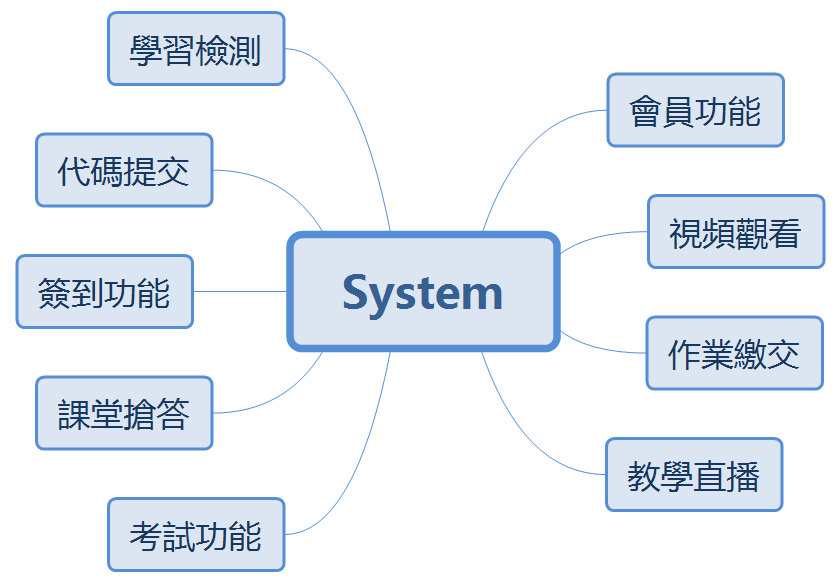
\includegraphics[width=0.50\textwidth]{ch1m1.png} 
\caption{期末作業系統架構規劃}
\label{Test}
\end{figure}

原系統設計是用 Python Flask 進行處理,當中整合當下前端框架 Vue 和深度學習框架 Pytorch,整個功能較為複雜,所以此次作業只是單純的驗證,人類臉部的狀態,也就是人的睜眼與眨眼狀況來進行判斷。一但有眨眼便會發起警告。

\begin{lstlisting}[language={python}]
if (由沒有人在鏡頭) {
    if (在鏡頭前的人有沒有可檢測的正臉) {
        if (眼睛的視線) {
            回傳
        }
        if (判斷人的表情是否為疲憊狀態) {
            回傳
        }
        回傳
    }
    回傳
}
\end{lstlisting}

J Cech 等人提出了一種實時檢測標準攝像機視頻序列中眨眼的算法,近期在野外數據集上訓練的地標檢測器對相機的頭部方向、不同的照明和麵部表情表現出出色的魯棒性,該研究表明,地標的檢測足夠精確,可以可靠地估計眼睛張開的水平。因此,所提出的算法估計地標位置,提取單個標量 - 眼睛縱橫比 EAR - 表徵每幀中的眼睛張開。最後,SVM 分類器將眨眼檢測為短時間窗口中的 EAR 值模式。其簡單的算法在兩個標準數據集上優於最先進的結果。

根據該篇論文,人臉關鍵點檢測中人眼共有 6 個關鍵點,睜眼時與閉眼時的關鍵點狀態如下圖,該篇研究提出了這個公式:

\begin{equation}
\mathrm{EAR}=\frac{\left\|p_{2}-p_{6}\right\|+\left\|p_{3}-p_{5}\right\|}{2\left\|p_{1}-p_{4}\right\|}
\end{equation}

通過該公式的歐氏距離計算,我們可以得到某一幀中眼睛是睜開還是閉著的狀態。計算左眼和右眼的平均 EAR 值,若 EAR 值小於某一閾值,則表明了這個人在某一幀中是睜眼還是閉眼的狀態。設定閾值 n ,連續 n 幀中若眼睛都是閉著的狀態,那麼代表這個人眨了一次眼。

\begin{figure}[H]
\centering 
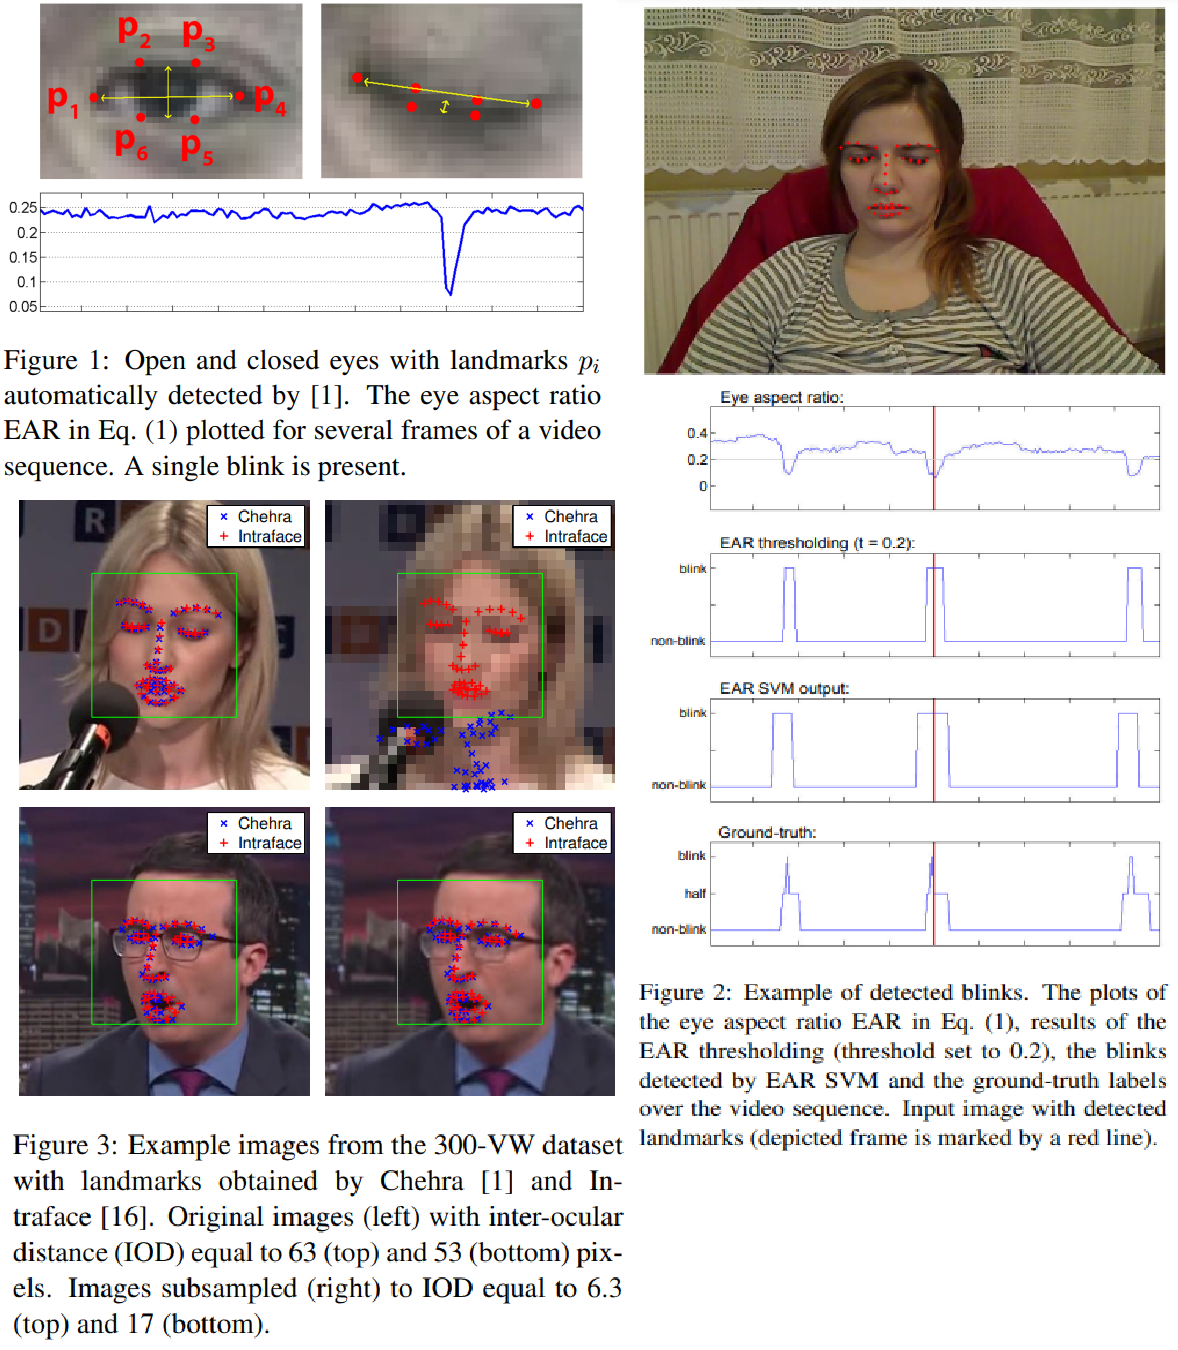
\includegraphics[width=0.90\textwidth]{ch3m1.png} 
\caption{期末作業文獻支持}
\label{Test}
\end{figure}

\newpage
\section{成果展示}

從下面的測試資料中可以看到,鏡頭前的人臉在閉上眼睛時畫面會跳出警告的訊息,而睜開眼睛則能夠看到當下是安全的文字訊息。當中綠色方框為人的臉部,而紅點所圈起的結構則是人的五官結構。

\begin{figure}[H]
\centering 
\includegraphics[width=0.80\textwidth]{fatigue-monitoring-sys-0.png} 
\caption{人臉閉眼狀態}
\label{Test}
\end{figure}

\begin{figure}[H]
\centering 
\includegraphics[width=0.80\textwidth]{fatigue-monitoring-sys-1.png} 
\caption{人臉開眼狀態}
\label{Test}
\end{figure}


%\section{附錄}

% 數學意義說明

% $$\min \limits_{G}\max \limits_{D}{V_I(D,\ G)=V(D,G)-\lambda L_I(G,Q)}$$

%	\begin{lstlisting}[language={python}]

%	\end{lstlisting}

%\begin{enumerate}
%\item Y
%\item A
%\end{enumerate}

% \newpage

\clearpage

\end{document}